\section{Troubleshooting and Testing}
During our project, we encountered various challenges that required creative problem-solving to keep things moving. Whether it was soldering mistakes, power-related issues, or flaws in the physical design, no prototype is perfect on the first try. This section outlines the key problems we faced during development, how we addressed them, and what test we performed on the prototypes. this section will also discuss things we couldn't get working exactly how we wanted and what steps should be taken to fix them.
\subsection{PCB and Power}
When designing the PCB, we considered several chip options but ultimately settled on the TPS563200. This chip was selected using the WEBENCH Power Designer. This software allows you to pick an input voltage, desired output voltage, and current, and then generate possible chips and schematics. This allowed us to generate some simulation files like the one seen in Fig. \ref{fig:Vout}. This shows a simulated start-up using this chip. R1 is selected so that \(V_{\text{out}}\) is 5V, and as you can see from the simulation, that is exactly what we got.
\begin{figure}[H]
    \centering
    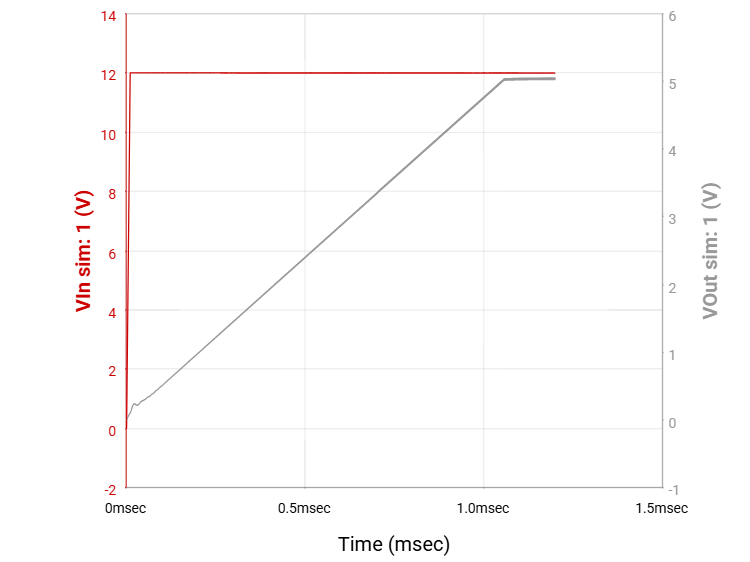
\includegraphics[height=6cm]{Vout_chart.png}
     \caption{Simulated Start up for the TPS563200}
    \label{fig:Vout}
\end{figure}
The DC-DC converter PCB was one of the many problems we had to overcome. The main issue was that the PCB successfully worked at larger loads($20~\Omega$), which drew around 0.25 amps. However, when we decreased the load to $3.5~\Omega$, drawing around 1.5A, the chip would burn out. After looking at potential issues ranging from lack of inrush current protection, voltage spikes, etc., the actual issue turned out to be the lack of a \(V_{\text{out}}\) copper pour between the inductor and output capacitors. The copper pour allows for good heat dissipation within the circuit, and since we didn't have any, the chip would overheat at low loads. We tried a couple of quick fixes like soldering more connections between the output capacitors and the inductor or increasing output capacitance. These solutions would hold the voltage for a little longer, up to around one minute, but ultimately they would burn up. So we switched to a voltage regulator, which, although it has a lower output current, was still sufficient to operate the servo and power the SpeedyBee. A long-term fix for using a DC-DC converter would be to redesign the PCB with a \(V_{\text{out}}\) pour to allow for better heat dissipation.
\subsection{Motor Operation and Grounding}
The main motor used for propulsion was one of the first challenges we had to overcome when dealing with the construction of our ASV. We purchased our motor with an ESC already included, which allowed us to control the motor with just power and a PWM signal wire. However, when trying to power our motor, we had trouble with the initial start. The way to fix this issue was to make sure everything had a common ground. Soldering the Raspberry Pi, SpeedyBee, and battery grounds together ensures no ground is floating, and we can get a clean signal to our motor from the SpeedyBee. In the future, a custom PCB with a shared ground rail would be the most effective way to ensure all grounds are the same, and save the most amount of space instead of soldering all the grounds together. 
\subsection{Physical Construction and Design}
Physical construction came with many unforeseen challenges, especially since the majority of our group specialized in electrical design and coding. One of the main issues we ran into was selecting what kind of material to make the base of our ASV with. The original plan was to make the base of the ASV out of acrylic. This would provide a lightweight base and allow us to laser cut or drill through it so we could attach things like the motor flange and our coil. However, when constructing our ASV, the acrylic sheet snapped under the tension of our coil while we were trying to drill the 1" hole for the motor connection. This made us switch to polycarbonate, which is slightly more flexible but is easier to drill through and cut. We also added MDF wood to give the base of the ASV a little more strength. In the future, teams should try and look to replace the MDF wood with something a little more secure and lightweight. Also, if future groups decide to go back to acrylic, the base case to cut through it is to laser cut all the holes for better precision. 